\chapter{DATA DESCRIPTION AND EXPLORATORY ANALYSIS}
\label{ch:data-description}

This chapter outlines the data collection, feature engineering, and integration procedures used to model cryptocurrency pump-and-dump events. Given the cross-platform nature of market manipulation, the dataset integrates social media signals, high-frequency trading metrics, and additional market-level data.

\section{Telegram Data Collection, Classification, and Event Aggregation}
\label{sec:telegram-collection}
\label{sec:message-classification}

Social media data was sourced from Telegram, one of the main platforms used to coordinate cryptocurrency pump-and-dump schemes \cite{li2021cryptocurrency}.

Historical messages were extracted via the Telethon Python library \cite{telethon2023}. Initial channels were identified via keyword searches for established manipulation terminology, isolating hundreds of potential sources. The dataset was subsequently expanded by tracing forwarded messages and incorporating channel references from prior literature (e.g., \cite{kamps2018pump, li2021cryptocurrency}), yielding an initial list of 336 channels.

Filtering for inactive, non-English, or unrelated to crypto pump-and-dump schemes reduced this list to 81 active pump channels. Event distribution across these channels is highly concentrated, with a small number of large groups accounting for most events, while the remaining channels account for a smaller number of events (see Figure~\ref{fig:channel-distribution} and Table~\ref{tab:top-channels}). This concentration describes channel activity, not necessarily stronger or more successful pump outcomes.

\begin{figure}[H]
    \centering
    \caption{Distribution of pump events across 81 Telegram channels.}
    \label{fig:channel-distribution}
    
\includegraphics[width=0.80\textwidth]{channel_distribution.pdf}
    \datasetsource
\end{figure}

\begin{table}[H]
\centering
\caption{Top 10 Most Active Pump Channels}
\label{tab:top-channels}
\begin{tabular}{|c|l|r|}
\toprule
\multicolumn{1}{|c|}{\textbf{Rank}} & \multicolumn{1}{c|}{\textbf{\textit{Channel ID}}} & \multicolumn{1}{c|}{\textbf{Event Count}} \\
\midrule
1 & 1167785945 & 367 \\
2 & 1195248520 & 346 \\
3 & 1151387276 & 231 \\
4 & 1174077730 & 229 \\
5 & 1093396548 & 211 \\
6 & 1198929017 & 209 \\
7 & 1122577430 & 204 \\
8 & 1211795583 & 195 \\
9 & 1217177161 & 140 \\
10 & 1123236170 & 102 \\
\bottomrule
\end{tabular}
\datasetsource
\end{table}

Isolating actionable pump signals from millions of standard chat messages created a need for a multi-stage filtering pipeline. Initially, keyword matching against 2,847 established coin and exchange names filtered the raw corpus of 12.4 million messages to 847,000 relevant candidates.

A subset of these candidates was classified into three categories (Table~\ref{tab:message-categories}) with the assistance of an LLM (Large Language Model), specifically Gemini 2.5 Pro \cite{gemini2025pro}. Utilizing such an advanced LLM for this initial annotation is an effective approach because correctly interpreting cryptocurrency pump signals requires parsing complex, unstructured text characterized by platform-specific slang, emojis, and erratic formatting. However, deploying a commercial LLM for the entire corpus presents significant limitations, most notably the financial cost of API (Application Programming Interface) access and the reliance on an external service with rate limits. To overcome these constraints, the Gemini-labeled subset was used as the training corpus for a fine-tuned XLM-RoBERTa model \cite{conneau2020xlmroberta}. XLM-RoBERTa is a multilingual transformer architecture selected for its strong cross-lingual performance and its ability to run as a local model after fine-tuning. This fine-tuned local model was subsequently used to classify the full candidate pool, enabling the scalable identification of pump-related messages across the entire dataset.

\begin{table}[H]
\centering
\caption{Message Classification Categories}
\label{tab:message-categories}
\begin{tabular}{|l|l|p{8.5cm}|}
\toprule
\multicolumn{1}{|c|}{\textbf{Category}} & \multicolumn{1}{c|}{\textbf{Label}} & \multicolumn{1}{c|}{\textbf{Description}} \\
\midrule
Explicit & 1 & The primary pump signal, containing the target coin symbol and execution instructions. \\
Preparatory & 2 & Countdowns and promotional messages designed to build anticipation prior to the coin reveal. \\
Noise & 0 & General discussion, market news, or unrelated spam. \\
\bottomrule
\end{tabular}
\ownsource
\end{table}



After message-level scoring, individual messages were grouped into distinct pump sessions using a 12-hour window so that closely related countdown and reveal messages stayed in the same event. Table~\ref{tab:session-example} illustrates an example session progressing from a countdown to the target coin reveal.

\begin{table}[H]
\centering
\caption{Example Pump Session: REQ/BTC Pump on March 27, 2021}
\label{tab:session-example}
\begin{tabular}{|l|p{10cm}|}
\toprule
\multicolumn{1}{|c|}{\textbf{Time}} & \multicolumn{1}{c|}{\textbf{Message Content}} \\
\midrule
18:25 & [megaphone] THE PUMP STARTS IN 5 MINUTES! \\
18:28 & [megaphone] 2 MINUTES - HAVE YOUR BTC READY ON BINANCE \\
18:29 & [clock] 1 minute... next message is the coin! \\
18:30 & [rocket x3] THE COIN IS: \#REQ [ROCKET x3] BUY ON BINANCE: REQ/BTC TARGET: +50\% \\
18:33 & [money] Up 8\%! KEEP GOING! \\
18:40 & [warning] Peak reached SELLING NOW! \\
\bottomrule
\end{tabular}
\datasetsource
\end{table}

The primary temporal marker for each session is $T_0$, which denotes the exact minute of the target asset's reveal. Every candidate $T_0$ was contextually verified also using Gemini 2.5 Pro, as subsequent volatility and return calculations are highly sensitive to timing accuracy. This process identified the initial actionable signal, whether a scheduled launch, an explicit coin announcement, or a direct trading instruction, to establish a precise starting point. The validation procedure confirmed or corrected 3,793 of the 3,876 candidate events (97.9\%), with 83 cases excluded due to inadequate signal clarity. These 3,793 validated events formed the event set before the later complete-case restrictions described in Section~\ref{sec:data-integration-summary}.

\section{Market Data Extraction, Asset Metadata, and Thin Market Constraints}
\label{sec:market-extraction}
\label{sec:metadata-constraints}

To quantify the market impact of the Telegram signals, 1-minute OHLCV data was retrieved around each $T_0$ timestamp. These historical records were acquired via the CCXT Python library \cite{ccxt2023} from four (still operating) cryptocurrency exchanges, including Binance, BitMEX, Bybit, and KuCoin. Binance served as the dominant target venue, accounting for 87.4\% of the events in the sample.

The extraction window for each event spans from seven days prior to the signal until one day after. Table~\ref{tab:ohlcv-example} shows one example of the market reaction at $T_0$. In this example, subdued prior trading activity is followed by a severe concurrent spike in price and volume at the reveal minute, and then by an immediate reversal.

\begin{table}[H]
\centering
\caption{Price and Volume Dynamics around NAS/BTC Pump ($T_0$ = 17:00 UTC)}
\label{tab:ohlcv-example}
\begin{tabular}{|l|l|l|l|l|l|}
\toprule
\multicolumn{1}{|c|}{\textbf{Time (UTC)}} & \multicolumn{1}{c|}{\textbf{Open}} & \multicolumn{1}{c|}{\textbf{High}} & \multicolumn{1}{c|}{\textbf{Low}} & \multicolumn{1}{c|}{\textbf{Close}} & \multicolumn{1}{c|}{\textbf{Volume}} \\
\midrule
16:58 & 0.00001310 & 0.00001320 & 0.00001300 & 0.00001310 & 21,217 \\
16:59 & 0.00001320 & 0.00001330 & 0.00001310 & 0.00001320 & 19,468 \\
17:00 & 0.00001320 & 0.00003240 & 0.00001320 & 0.00002000 & 12,309,246 \\
17:01 & 0.00002000 & 0.00002070 & 0.00001440 & 0.00001730 & 3,861,392 \\
\bottomrule
\end{tabular}
\datasetsource
\end{table}


On cryptocurrency exchanges, altcoins are typically quoted against a small set of liquid reference assets. In this dataset, the main quote currencies are BTC, ETH, BNB, and USDT (Tether). BTC and ETH represent crypto-denominated trading pairs, meaning that the target coin is priced against another volatile cryptocurrency. USDT, by contrast, is a stablecoin pegged to the US dollar, so USDT pairs make the \textit{10-Minute Logarithmic Return} easier to interpret in dollar terms and reduce exposure to BTC or ETH price movements during the event \cite{tether2026howitworks}. BNB appears in the sample because some observed Binance markets used Binance's native ecosystem token as the quote asset. Binance provides users with practical reasons to hold BNB, including cheaper trading \cite{binanceus2026bnbfees}, access to rewards, gas usage on the BNB Chain, as well as staking and governance rights \cite{binanceacademy2025bnb}. These utility features help explain why BNB appears as a quote currency in the extracted market data.

Figure~\ref{fig:quote-currency-temporal} shows how the composition of these quote currencies evolved within the thesis sample over the 2019 to 2021 period, which concentrates the majority of observed events. In early 2019, BTC-denominated pairs accounted for over 80\% of pump targets, showing that BTC was the dominant reference asset in the most event-concentrated periods of the sample. This historical dominance established the data extraction rule for ambiguous signals. When a message named only the target coin without specifying the quote currency (e.g., NAS instead of NAS/USDT or NAS/BTC), the BTC pair was assigned as the default to maintain consistency. By mid-2020, USDT pairs had become the dominant quote currency among observed events. This later shift may be related to USDT becoming more widely used as a liquid exchange trading pair \cite{tether2026exchanges}.

\begin{figure}[H]
    \centering
    \caption{Quarterly share of pump events by quote currency (2019 to 2021).}
    \label{fig:quote-currency-temporal}
    
\includegraphics[width=0.95\textwidth]{quote_currency_temporal_v2.pdf}
    \datasetnote{Figure limited to 2019--2021.}
\end{figure}

Each targeted token was additionally enriched with project metadata from CoinMarketCap \cite{coinmarketcap2024api}. To prevent the pump from distorting these attributes, the metadata was extracted from historical snapshots recorded on the Sunday preceding each event.

Two key variables used later as pre-reveal covariates are \textit{Coin Age} and \textit{Market Capitalization}. \textit{Coin Age} was computed from exchange listing dates, while \textit{Market Capitalization} was taken from the historical CoinMarketCap snapshot. The historical CoinMarketCap 24-hour trading-volume field is transformed into \textit{log\_cmc\_volume\_24h}, the natural logarithm of that volume, before use. Figure~\ref{fig:coin-age-distribution} shows that many targets were several hundred to about 1,000 days old, while very new listings were less common. Figure~\ref{fig:market-cap-volume-scatter} shows that targets cluster most heavily in the 10 million USD (US dollars) to 1 billion USD market-cap range.

\begin{figure}[H]
    \centering
    \caption{Distribution of target \textit{Coin Age} at $T_0$.}
    \label{fig:coin-age-distribution}
    
\includegraphics[width=0.80\textwidth]{coin_age_distribution.pdf}
    \datasetnote{The x-axis uses a log scale.}
\end{figure}

\begin{figure}[H]
    \centering
    \caption{Pump targets by historical \textit{Market Capitalization} and total 24-hour trading volume.}
    \label{fig:market-cap-volume-scatter}
    
\includegraphics[width=0.85\textwidth]{market_cap_volume_scatter.pdf}
    \datasetnote{}
\end{figure}

Many of these targeted crypto projects fail or are delisted, creating a data-availability problem for historical analysis. Restricting the analysis to currently active listings would therefore create survivorship risk in the final sample. To reduce this problem, the study uses historical exchange data so that tokens no longer actively listed can still be retained when data is available.

The metadata also reveals severe trading sparsity among the lowest-cap observations. For coins below 10 million USD in \textit{Market Capitalization}, over 68\% of the 1-minute intervals before the pump recorded zero trading volume. For that reason, subsequent volatility metrics are computed only across intervals with non-zero trading volume.

\section{Variable Construction and Formal Specifications}
\label{sec:feature-selection}

Following data integration, features were engineered to support the causal and predictive analyses. To keep pre-reveal covariates separate from post-signal outcomes, all feature construction strictly respected the $T_0$ temporal threshold.

Telegram signal features quantify the scale and intensity of social coordination (Table~\ref{tab:telegram-variables}). The engineered feature set includes \textit{Hype Volume}, \textit{Hype Intensity}, \textit{Urgency Index}, and \textit{Instruction Density}. Chapter~\ref{ch:methodology} defines which of these variables enter the causal treatment vector. \textit{Hype Volume} remains part of the engineered signal-feature set for predictive modeling, but is not used as a causal treatment.

\begin{table}[H]
\centering
\caption{Engineered Telegram Signal Features}
\label{tab:telegram-variables}
\begin{tabular}{|l|p{11cm}|}
\toprule
\multicolumn{1}{|c|}{\textbf{Variable}} & \multicolumn{1}{c|}{\textbf{Description}} \\
\midrule
\textit{Hype Volume} & The absolute number of preparatory messages broadcasted in the 20-minute window immediately preceding the coin reveal. \\
\textit{Hype Intensity} & The ratio of messages transmitted in the final 20 minutes prior to $T_0$ relative to all earlier preparatory messages in the session, capturing pre-reveal acceleration. \\
\textit{Urgency Index} & The ratio of uppercase alphabetic characters to all alphabetic characters in the primary signal message, used in this thesis as a simple proxy for urgency-style message framing. \\
\textit{Instruction Density} & The word count of the signal message, reflecting the complexity of the trading instructions. \\
\bottomrule
\end{tabular}
\ownsource
\end{table}

Pre-reveal market covariates capture the state of the market immediately before the public coin reveal at $T_0$. These metrics are computed over trailing intervals ending precisely at $T_0 - 1$ minute, ensuring they reflect strictly pre-reveal market conditions. Here, $T_0-k$ denotes $k$ minutes before the reveal. Depending on the metric's theoretical purpose, the observation window spans the preceding 30 minutes for localized microstructure dynamics, 60 minutes for immediate run-up and abnormal volume detection, or 24 hours for baseline structural properties.

Pre-event volatility measures short-horizon price variability over the trailing 30 minutes and is computed only during intervals with active trading:
\begin{equation}
    \label{eq:pre_vol}
    \sigma_{\text{pre}} = \mathrm{Std}\!\left(\{r_i\}_{i \in [T_0-31,\, T_0-1],\, V_i > 0}\right)
\end{equation}
where $\mathrm{Std}$ denotes the standard deviation, $r_i$ denotes the 1-minute logarithmic return, representing the relative price change between consecutive observations normalized for statistical stability, and $V_i$ is the trading volume at minute $i$. The set notation keeps only pre-reveal minutes with positive volume. The window contains 31 possible close-price observations, which produce up to 30 logarithmic returns after inactive candles are removed.

The volume z-score captures abnormal trading volume at $T_0 - 1$, designed to detect potential insider front-running prior to the public announcement \cite{lamorgia2020pump}:
\begin{equation}
    \label{eq:vol_z_score}
    Z_V = \frac{V_{T_0-1} - \bar{V}_{[T_0-61,\, T_0-1]}}{\sigma_{V_{[T_0-61,\, T_0-1]}}}
\end{equation}
where $V_{T_0-1}$ is the trading volume one minute prior to the signal, $\bar{V}$ is the 60-minute rolling mean volume, and $\sigma_V$ is the corresponding rolling standard deviation over the same window. If the rolling standard deviation is zero, the z-score is set to 0.

Baseline illiquidity is quantified via the median Amihud illiquidity ratio computed over the preceding 24 hours, establishing the baseline price impact of standard market activity \cite{amihud2002illiquidity}:
\begin{equation}
    \label{eq:baseline_illiq}
    \lambda_{\text{base}} = \operatorname{median}_{t \in [T_0-24\text{h},\, T_0-1]} \left( \frac{|r_t|}{V_t \times P_t} \right)
\end{equation}
where $r_t$ is the one-minute percentage return, $V_t$ is the volume, and $P_t$ is the closing price at minute $t$. The product $V_t \times P_t$ is the traded value in the quote currency. Candles with zero volume are excluded, and infinite ratios are treated as missing.

In addition to baseline confounders, a set of high-frequency microstructure features capture fine-grained market conditions and potential pre-pump anomalies in the rolling 30 to 60 minutes immediately preceding the pump.

The pre-pump run-up measures the cumulative logarithmic return over the 60 minutes preceding the signal:
\begin{equation}
    \label{eq:pre_run_up}
    R_{\text{up}} = \ln \left( \frac{P_{T_0-1}}{P_{T_0-61}} \right)
\end{equation}
where $P_{T_0-1}$ is the closing price immediately before the pump and $P_{T_0-61}$ is the closing price one hour prior. Elevated values may be consistent with early activity before the public announcement, including possible accumulation or information leakage \cite{lamorgia2020pump}.

The Roll spread serves as an estimate for the effective bid-ask spread, the cost potentially incurred when executing a trade. This measure approximates the spread by analyzing the serial covariance of close-price differences, capturing the "bounce" effect of trades as they hit the bid or ask prices \cite{roll1984simple}. It is computed over the 30-minute pre-pump window:
\begin{equation}
    \label{eq:roll_spread}
    S_{\text{Roll}} = 2\sqrt{-\mathrm{Cov}(\Delta P_t,\, \Delta P_{t-1})}
\end{equation}
where $\Delta P_t$ is the one-minute close-price difference, and $\mathrm{Cov}(\Delta P_t, \Delta P_{t-1})$ is the sample autocovariance between the current and previous close-price differences over the 30-minute pre-pump window. The measure is defined only when this covariance is negative. Otherwise it is set identically to zero.

The log-transformed Amihud illiquidity ratio is additionally evaluated over the immediate 30-minute pre-pump window to capture localized liquidity conditions:
\begin{equation}
    \label{eq:short_illiq}
    \lambda_{\text{short}} =
    \log\!\left(
    \operatorname{mean}_{t \in [T_0-30,\, T_0-1]}
    \frac{|r_t|}{V_t \times P_t}
    + 10^{-9}
    \right)
\end{equation}
where $r_t$, $V_t$, and $P_t$ denote the one-minute percentage return, volume, and close price, respectively. The small constant $10^{-9}$ avoids taking the logarithm of zero. As with the baseline Amihud measure, zero-volume candles are excluded before calculating the mean, and infinite ratios are treated as missing. Because the logarithm is applied to the mean illiquidity value plus this small constant, negative values can occur when the mean is below 1. This localized variant ($\lambda_{\text{short}}$) complements the 24-hour baseline illiquidity ratio ($\lambda_{\text{base}}$) by differentiating between structural illiquidity over a full day and local liquidity conditions in the 30 minutes before the pump signal.

The CLV (Close Location Value) summarizes where the close falls within each 1-minute candle \cite{ulrich2024clv}:
\begin{equation}
    \label{eq:clv}
    \overline{\text{CLV}} = \frac{1}{30} \sum_{t=T_0-30}^{T_0-1} \frac{(C_t - L_t) - (H_t - C_t)}{H_t - L_t}
\end{equation}
where $H_t$, $L_t$, and $C_t$ denote the highest, lowest, and closing prices during minute $t$. Values approaching $+1$ indicate consistent closing near the high (buying pressure), while values near $-1$ indicate closing near the low (selling pressure). If $H_t=L_t$, the candle has no price range and its CLV term is set to 0 before averaging.

Parkinson volatility is a range-based estimator that captures intracandle price variance often unobservable via standard close-to-close returns \cite{parkinson1980extreme}:
\begin{equation}
    \label{eq:parkinson}
    \sigma_{\text{Park}} = \sqrt{\frac{1}{4 \ln 2 \cdot 30} \sum_{t=T_0-30}^{T_0-1} \!\left( \ln \frac{H_t}{L_t} \right)^{\!2}}
\end{equation}
where $H_t$ and $L_t$ are the high and low prices during minute $t$.

The zero return ratio captures the proportion of 1-minute intervals recording no price change:
\begin{equation}
    \label{eq:zero_ret}
    \rho_0 = \frac{1}{30} \sum_{t=T_0-30}^{T_0-1} I[r_t = 0]
\end{equation}
where $I[\cdot]$ is the indicator function, evaluating to 1 when the return $r_t$ is exactly zero and 0 otherwise. Higher values indicate more frequent price staleness and are interpreted in the empirical framework as evidence of thinner trading conditions.

Beyond market metrics, temporal scheduling was encoded via \textit{is\_weekend}. This binary variable equals 1 if $T_0$ falls on a Saturday or Sunday, and 0 otherwise. It is included to absorb weekend-specific differences in market conditions and trading behavior.

Finally, the preliminary synthetic-control stage, discussed in the appendix, produced two hold-out fit diagnostics per event. These were the coefficient of determination, reported as \textit{Hold-Out} $R^2$, and \textit{Root Mean Square Error}. These variables were originally used as quality checks to see how accurately the synthetic control matched the target coin's price path before the pump. However, they are also kept in the integrated dataset as extra features for the classification models. This helps test if pre-event price patterns contain information about post-signal pump \textit{Success}.

\section{Integrated Sample and Exploratory Patterns}
\label{sec:data-integration-summary}

The data compilation pipeline unifies unstructured Telegram chat logs, high-frequency OHLCV arrays, and historical CoinMarketCap metadata. The architectural workflow of this integration is mapped in Figure~\ref{fig:data-pipeline-overview}.

\begin{figure}[H]
    \centering
    \caption{Data integration architecture for the event matrix.}
    \label{fig:data-pipeline-overview}
    \begin{tikzpicture}[
        node distance=1.5cm,
        box/.style={rectangle, draw, rounded corners, minimum width=3cm, minimum height=1cm, align=center, font=\small},
        arrow/.style={-{Stealth[length=3mm]}, thick}
    ]
        % Source nodes
        \node[box, fill=blue!20] (telegram) {Telegram\\Messages\\(12.4 million raw)};
        \node[box, fill=green!20, right=of telegram] (ohlcv) {Exchange\\OHLCV\\(4 exchanges)};
        \node[box, fill=orange!20, right=of ohlcv] (cmc) {CoinMarketCap\\API\\(historical)};
        
        % Processing nodes
        \node[box, fill=gray!20, below=of telegram] (classify) {Classification\\Pipeline};
        \node[box, fill=gray!20, below=of ohlcv] (align) {Temporal\\Alignment};
        \node[box, fill=gray!20, below=of cmc] (enrich) {Metadata\\Enrichment};
        
        % Integration node
        \node[box, fill=purple!20, below=2cm of align, minimum width=4cm] (integrate) {Integrated Event Matrix\\(2,917 events)};
        
        % Arrows
        \draw[arrow] (telegram) -- (classify);
        \draw[arrow] (ohlcv) -- (align);
        \draw[arrow] (cmc) -- (enrich);
        \draw[arrow] (classify) -- (integrate);
        \draw[arrow] (align) -- (integrate);
        \draw[arrow] (enrich) -- (integrate);
    \end{tikzpicture}
    \ownsource
\end{figure}

The workflow separates Telegram classification, OHLCV alignment, and metadata enrichment before merging them into the final event matrix.

The final analytical sample consists of 2,917 complete pump-event records. Observations were excluded if any pre-reveal covariates were missing, ensuring that each event had the baseline market conditions required for causal estimation. The \textit{10-Minute Logarithmic Return} was then winsorized at the 1st and 99th percentiles to limit the influence of extreme price outliers. Table~\ref{tab:sample-distribution} shows the breakdown of this final sample across the four \textit{Market Capitalization} strata used in the stratified estimation.

\begin{table}[H]
\centering
\caption{Sample Distribution by \textit{Market Capitalization}}
\label{tab:sample-distribution}
\begin{tabular}{|l|r|r|}
\toprule
\multicolumn{1}{|c|}{\textbf{\textit{Market Capitalization Stratum}}} & \multicolumn{1}{c|}{\textbf{Number of Events}} & \multicolumn{1}{c|}{\textbf{\%}} \\
\midrule
Micro ($<$10M USD) & 289 & 9.9\% \\
Small (10M USD--100M USD) & 1{,}182 & 40.5\% \\
Mid (100M USD--1B USD) & 967 & 33.2\% \\
Large ($>$1B USD) & 479 & 16.4\% \\
\midrule
Total & 2{,}917 & 100.0\% \\
\bottomrule
\end{tabular}
\datasetsource
\end{table}

The final sample is concentrated in small- and mid-cap assets, with the 10 million USD to 1 billion USD stratum forming the largest group.

To illustrate what a single row in the integrated dataset looks like, Table~\ref{tab:sample-observations} presents four sampled observations from the integrated event matrix. Each coin represents a separate blockchain-based software project that has issued its own tradeable token. DOCK, for example, provides infrastructure for issuing and verifying digital credentials such as diplomas or professional certificates, reducing the need for direct contact with the issuing organization \cite{dock2026dids}. RLC (iExec) is linked to a network where the token is used to access computing resources and related digital assets \cite{iexec2025tokenomics}. TRB (Tellor) acts as a data relay because blockchain applications cannot access information from the outside world on their own. Tellor lets reporters submit external data and uses staking and dispute mechanisms to discourage false reporting \cite{tellor2026fundamentals, tellor2026disputes}. RVN (Ravencoin) allows users to create custom digital assets that can represent real-world or digital assets, such as security tokens, digital art, real estate, gem stones, wine futures, or in-game currency \cite{ravencoin2026assets}. More broadly, such token-based projects often issue tokens to finance platform development and to reward users or contributors who provide resources to the network \cite{cong2022tokenbased}. Each row in the table contains asset metadata, Telegram signal features, pre-reveal market covariates, the primary outcome, and synthetic control fit diagnostics. In the outcome row, $Y_{10}$ denotes the logarithmic return from $T_0$ to $T_0+10$ minutes.

\begin{table}[H]
\centering
\caption{Sample Observations from the Integrated Event Matrix}
\label{tab:sample-observations}
\small
\begin{tabular}{|l|r|r|r|r|}
\toprule
\textbf{Variable} & \textbf{DOCK} & \textbf{RLC} & \textbf{TRB} & \textbf{RVN} \\
\midrule
\multicolumn{5}{|l|}{\textit{Asset Metadata}} \\
\quad \textit{Market Capitalization Stratum} & Micro & Small & Small & Mid \\
\quad \textit{Market Capitalization} & 3.9M USD & 24.7M USD & 73.2M USD & 111.4M USD \\
\quad \textit{Coin Age} (days) & 518 & 829 & 483 & 417 \\
\midrule
\multicolumn{5}{|l|}{\textit{Telegram Signal Features (Table~\ref{tab:telegram-variables})}} \\
\quad \textit{Hype Volume} & 0 & 1 & 2 & 0 \\
\quad \textit{Hype Intensity} & 0.000 & 0.500 & 2.000 & 0.000 \\
\quad \textit{Urgency Index} & 0.426 & 1.000 & 0.240 & 0.215 \\
\quad \textit{Instruction Density} & 48 & 9 & 8 & 24 \\
\midrule
\multicolumn{5}{|l|}{\textit{Pre-Reveal Market Covariates}} \\
\quad $\sigma_{\text{pre}}$ {\footnotesize (Eq.~\eqref{eq:pre_vol})} & 0.0076 & 0.0021 & 0.0025 & 0.0045 \\
\quad $Z_V$ {\footnotesize (Eq.~\eqref{eq:vol_z_score})} & $-$0.023 & $-$0.284 & $-$0.299 & $-$0.734 \\
\quad $\lambda_{\text{base}}$ {\footnotesize (Eq.~\eqref{eq:baseline_illiq})} & 0.265 & 0.104 & 0.164 & 0.000 \\
\quad $R_{\text{up}}$ {\footnotesize (Eq.~\eqref{eq:pre_run_up})} & 0.011 & 0.008 & $-$0.001 & 0.017 \\
\quad $S_{\text{Roll}}$ {\footnotesize (Eq.~\eqref{eq:roll_spread})} & $\approx$0 & $\approx$0 & 0.001 & $\approx$0 \\
\quad $\lambda_{\text{short}}$ {\footnotesize (Eq.~\eqref{eq:short_illiq})} & $-$1.068 & 1.433 & $-$0.260 & $-$6.443 \\
\quad $\overline{\text{CLV}}$ {\footnotesize (Eq.~\eqref{eq:clv})} & $-$0.065 & 0.161 & $-$0.097 & $-$0.070 \\
\quad $\sigma_{\text{Park}}$ {\footnotesize (Eq.~\eqref{eq:parkinson})} & 0.0036 & 0.0012 & 0.0012 & 0.0048 \\
\quad $\rho_0$ {\footnotesize (Eq.~\eqref{eq:zero_ret})} & 0.516 & 0.742 & 0.645 & 0.387 \\
\midrule
\multicolumn{5}{|l|}{\textit{Outcome (Eq.~\eqref{eq:log-return})}} \\
\quad $Y_{10}$ (\textit{10-Minute Logarithmic Return}) & 0.011 & $-$0.017 & 0.001 & $-$0.011 \\
\midrule
\multicolumn{5}{|l|}{\textit{Synthetic Control Diagnostics (appendix)}} \\
\quad \textit{Hold-Out} $R^2$ & $-$0.001 & $-$0.066 & $-$0.024 & $-$0.048 \\
\quad \textit{Root Mean Square Error} (hold-out) & 0.008 & 0.002 & 0.001 & 0.002 \\
\bottomrule
\end{tabular}
\datasetsource
\end{table}

Figure~\ref{fig:outcome-distribution-mcap} further illustrates how the \textit{10-Minute Logarithmic Return}, the primary outcome variable defined in Section~\ref{sec:outcome-variable}, is distributed across these strata. The figure shows the central 95\% of observations. Micro- and small-cap assets display greater variance than the larger strata, which is consistent with the thin-market constraints discussed above.

\begin{figure}[H]
\centering
\caption{Distribution of \textit{10-Minute Logarithmic Return} by \textit{Market Capitalization Stratum}.}
\label{fig:outcome-distribution-mcap}
\begin{tikzpicture}
    \node[inner sep=0] (img) {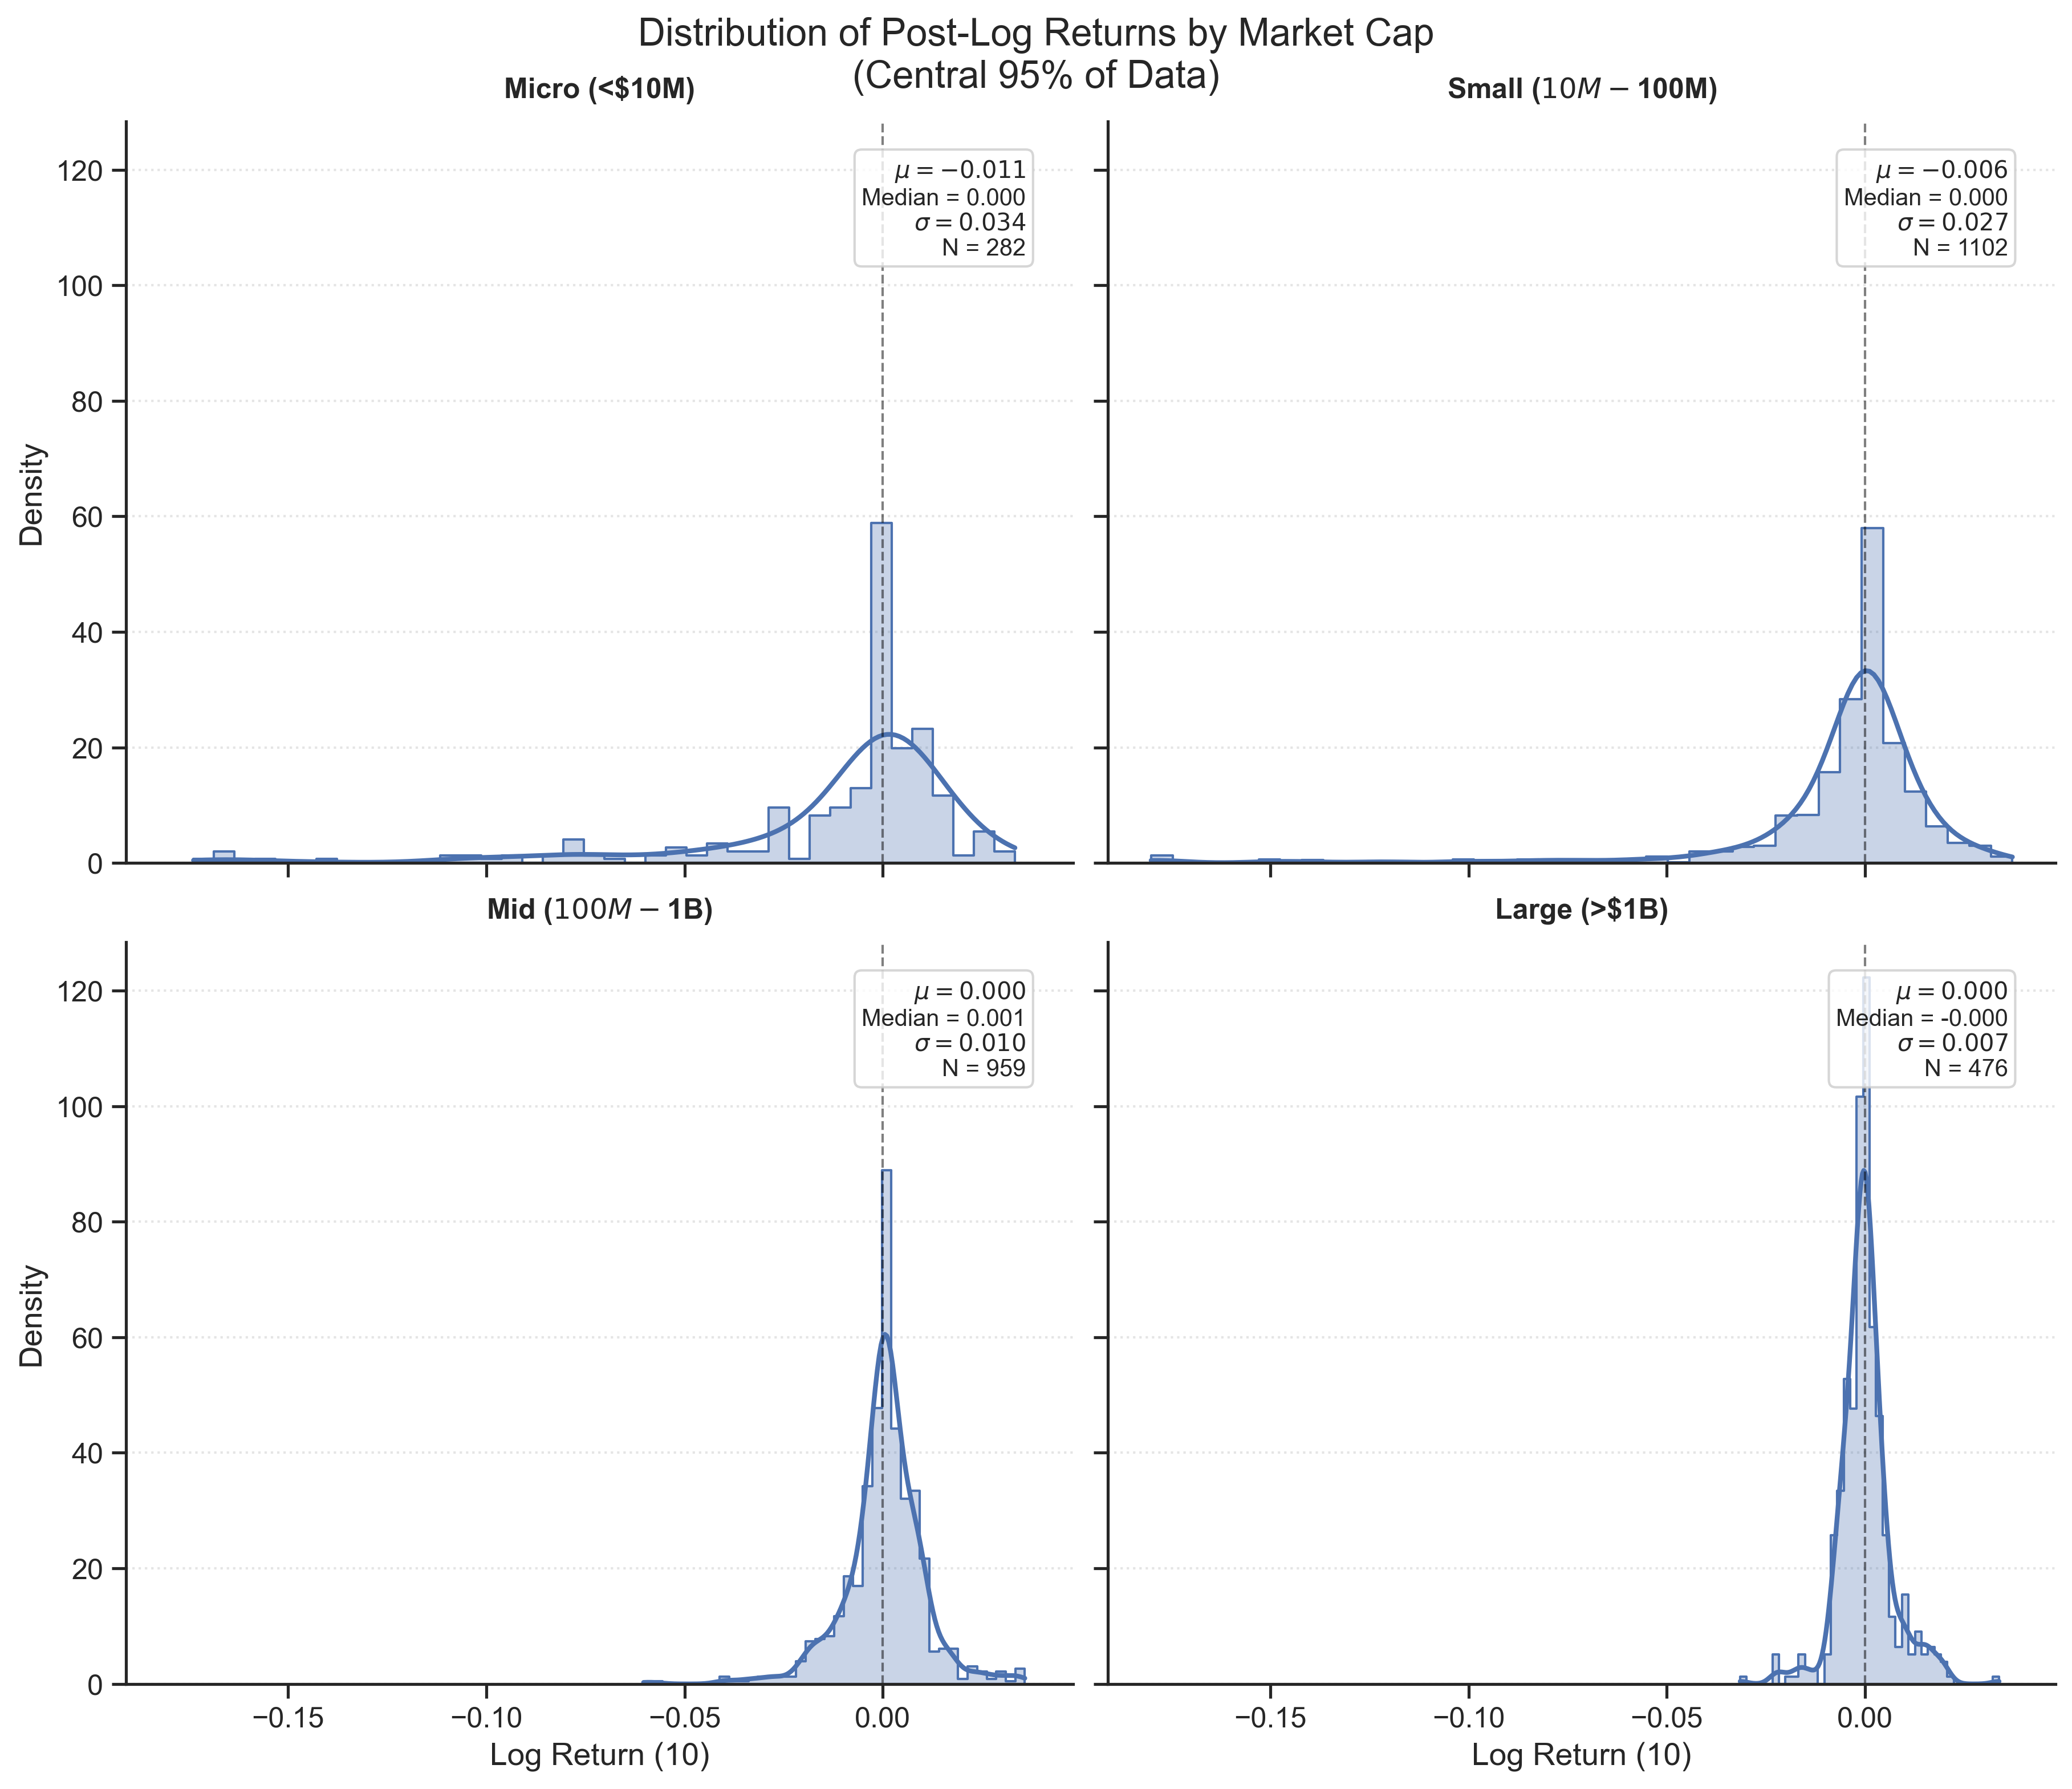
\includegraphics[width=\textwidth,trim=0 0 0 9mm,clip]{figures/ch4/outcome_distribution_by_mcap.png}};
    \fill[white] ([xshift=-2.9cm,yshift=0.02cm]img.north) rectangle ([xshift=2.9cm,yshift=-0.56cm]img.north);
\end{tikzpicture}
\datasetnote{Figure shows the central 95\% of observations; within each panel, $\mu$ denotes the mean, $\sigma$ denotes the standard deviation, and $N$ denotes the number of observations in the stratum; \textdollar{} denotes USD; M denotes million; B denotes billion.}
\end{figure}

Figure~\ref{fig:channel-returns-distribution} adds the channel-level perspective. Channels are sorted by their median \textit{10-Minute Logarithmic Return}, vertical lines show the interquartile range, colors mark whether the median is positive, and point size reflects the number of observed events. The chart shows that median outcomes differ across channels, but many high-volume channels remain close to zero. This suggests that channels differ in their typical outcomes.

\begin{figure}[H]
\centering
\caption{Channel-level \textit{10-Minute Logarithmic Return} distribution.}
\label{fig:channel-returns-distribution}

\includegraphics[width=\textwidth]{channel_returns_distribution.png}
\datasetnote{Orange points denote channels with median return $\leq 0$; green points denote channels with median return $> 0$; $N$ denotes the number of observed events for a channel and determines point size.}
\end{figure}

Together, these records supply the treatment variables, confounders, and price data required for the causal analysis in Chapter~\ref{ch:methodology}, with \textit{Market Capitalization} also serving as the stratification key in Section~\ref{sec:stratified-estimation}.
